% 2010 年辽宁卷理科第 15 题：网格纸上的三视图（正视图、侧视图、俯视图）。
% 来源 PDF：普通高考/2010/2010辽宁理.pdf，SHA-256 ba46f70f9d718652c24d14b28a0b473b768e864248ff0a9f1feb2374aec708f9。
% 原页：第 1 页（A3 三栏）第 2 栏下部，书页码 611。
% 重绘依据：照原页 L 形网格——上块 8 列 × 4 行，左下块另起 4 列 × 3 行，共 7 行；
%   左上是正视图（直角边在右、下，斜边自左下至右上），右上是侧视图（直角边在左、下，
%   斜边自左上至右下），左下是俯视图（正方形加一条自左下至右上的对角线）。
%   网格用细灰线，三视图轮廓用粗黑线。
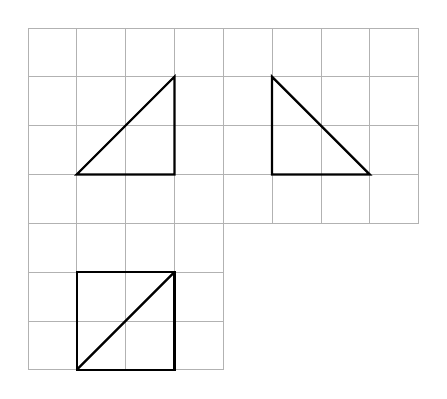
\begin{tikzpicture}[scale=0.62]
  % 网格：上块 8×4（y=3..7 满宽），左下块 4×3（y=0..3 仅左 4 列）
  \foreach \y in {0,1,2} {
    \draw[gray!60, very thin] (0,\y) -- (4,\y);
  }
  \foreach \y in {3,4,5,6,7} {
    \draw[gray!60, very thin] (0,\y) -- (8,\y);
  }
  \foreach \x in {0,1,2,3,4} {
    \draw[gray!60, very thin] (\x,0) -- (\x,7);
  }
  \foreach \x in {5,6,7,8} {
    \draw[gray!60, very thin] (\x,3) -- (\x,7);
  }

  % 正视图（左上）：直角边 2、2，斜边自左下至右上
  \draw[thick] (1,4) -- (3,4) -- (3,6) -- cycle;
  % 侧视图（右上）：直角边 2、2，斜边自左上至右下
  \draw[thick] (5,4) -- (7,4) -- (5,6) -- cycle;
  % 俯视图（左下）：正方形加一条对角线
  \draw[thick] (1,0) rectangle (3,2);
  \draw[thick] (1,0) -- (3,2);
\end{tikzpicture}
